\subsection{Mixture approximation of the proteins distribution}

On one side, the transitions of the coarse-grained model described in Section \ref{meta_red} happen on a time scale which is expected to be of the order of $e^{\frac{C}{\varepsilon}}$, where $C$ is an unknown constant depending on the basins (owing to a Large deviations principle, as studied in \cite{ventre2020reduction}). For small $\varepsilon$, such transitions are then generally rare events, and it can be considered that the process spends in each basin a time long enough to equilibrate inside, \textit{i.e} that a cell reaches between each transition its stationary distribution knowing a basin. On the other side, the sigmoidal form \eqref{kon} for the functions $k_{on,i}^\theta$ implies that these functions must not vary significantly inside a basin: a rough approximation could lead to identify the bursts rate in each basin by its dominant rate inside, corresponding to the value of $k_{\mathit{on,i}}$ on the attractor $P_z$. For any gene $i=1,\cdots,n$ and any basin $z \in Z$, we can then approximate: 
$$\forall P \in z:\,k_{\mathit{on},i}^\theta(P) \approx k_{\mathit{on},i}^\theta(P_z).$$
This implies that the distribution of a cell knowing a basin can be approximated by the stationary distribution of a simpler model with constant burst rates, which appears as a product of $\textrm{Gamma}$ distributions \cite{mackey2011molecular}. We obtain the following approximation for the stationary distribution within each basin $z \in Z$: 
\begin{align*}
    \hat{u}_{z}^\theta \approx \prod\limits_{i=1}^n\textrm{Gamma}\left(\frac{k_{\mathit{on},i}^\theta(P_z)}{d_{1,i}},c_i\right),
\end{align*}

Finally, we can approximate the stationary distribution of the process associated to a given GRN $\hat{u}^\theta$ by a mixture of $\textrm{Gamma}$ distributions. Denoting for any $z \in Z,\, i=1,\cdots,n,\, k_{z, i} = k_{\mathit{on},i}^\theta(P_z)$, we obtain
\begin{align}
    \hat{u}^\theta \approx \hat{u}_\varepsilon = \sum\limits_{z \in Z}\mu(z)\prod\limits_{j=1}^n\textrm{Gamma}\left(\frac{k_{z, j}}{d_{1,j}},c_j\right),
    \label{dist:mixture}
\end{align}
where $\mu$ is the probability vector on the basins at the steady-state. In some sens, this approximation consists in reducing the dependence between genes resulting from the GRN to the coexistence and relative weight of different basins corresponding to the different existing modes of promoters frequency.\\

The heuristic analysis presented above then states that when the functions $k_{on,i}$ are close to constant functions inside the basins and that $\epsilon$ is small, the mixture approximation \eqref{dist:mixture} is a good approximation of the distribution $\hat{u}^\theta$. We remark that this is straightforward when the scaling factor $\varepsilon$ is close to $0$. Indeed, any GRN $\theta$ being associated to an unknown stationary distribution, that we denote $\hat{u}^\theta_\varepsilon$ and which converges to a sum of Dirac on the attractors when $\varepsilon \to 0$ \cite{papanicolaou1975asymptotic}, we see that the Gamma mixture $\hat{u}_\varepsilon$ converges to the same sum of Dirac when $\varepsilon \to 0$, as the mean of each Gamma does not depend on $\varepsilon$ while the variance is proportional to $\varepsilon$: $|\hat{u}^\theta_\varepsilon - \hat{u}_\varepsilon| \to 0$ as $\varepsilon \to 0$. When the noise $\varepsilon$ is not negligible, the problem is more complex and finding a theoretical bound for the quantity $|\hat{u}^\theta_\varepsilon - \hat{u}_\varepsilon|$, depending on $\varepsilon$, is beyond the scope of this paper. Nevertheless, we see in Figure \ref{fig:comp_mixture} that the Wasserstein distance between the empirical distribution associated to a proteins dataset simulated from the mechanistic model \eqref{model_final} and the Gamma mixture distribution \eqref{dist:mixture} is much smaller than the distance between the same dataset and a mixture of normal distribution (fitted with a Gaussian Mixture Model). This let us think that the Gamma mixture approximation is indeed close to the true distribution even when the weak noise limit assumption is not realistic (and that the distribution is far from a sum of Dirac).

\iffalse
\begin{figure}
\centering
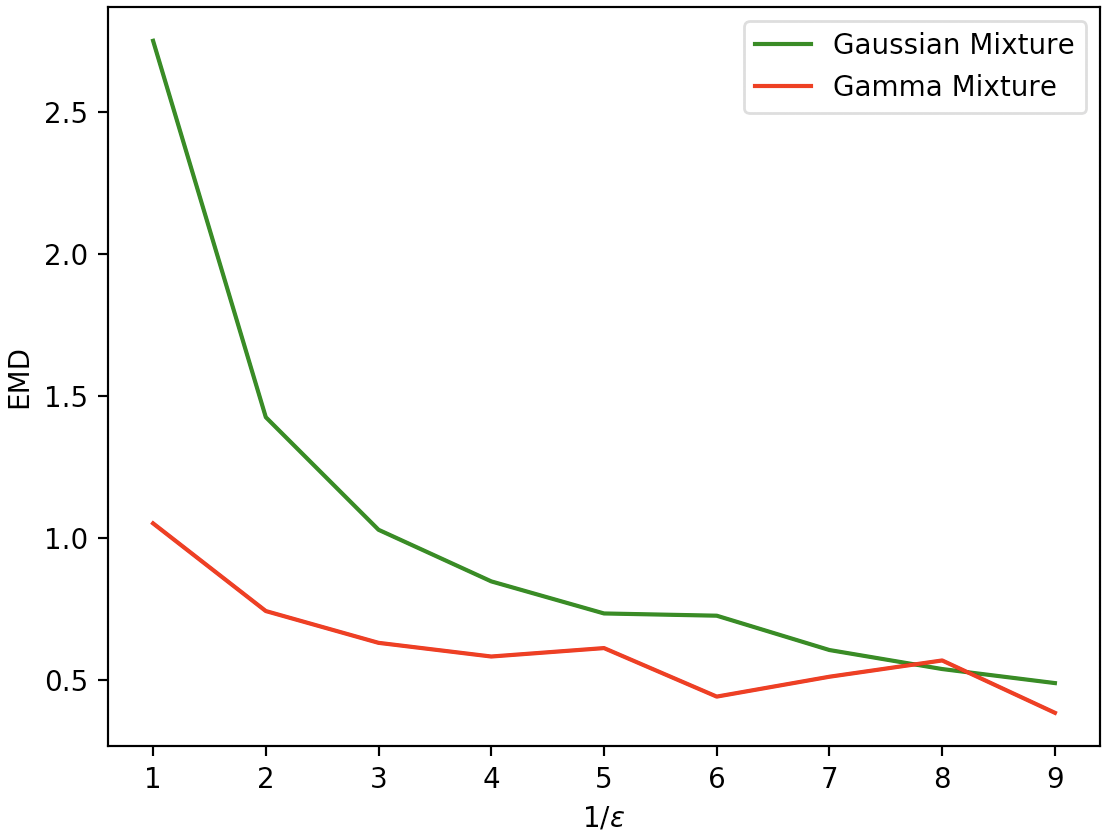
\includegraphics[width=7cm, height=5cm]{Images/comparison.png}
    \caption{Evolution in function of $1/\varepsilon$ of the Wasserstein distances between the empirical distribution associated to a set of $2000$ cells, simulated with the model \eqref{model_final}, and both the Gamma mixture approximation \eqref{dist:mixture} (in red) and a GMM approximation (in green), for the toggle-switch network described in Appendix \ref{Appendix_toggleswitch}.}
    \label{fig:comp_mixture}
\end{figure}
\fi

\subsection{Linking a GRN to mixture parameters}

Building an analytical link between the GRN and the mixture parameters is generally out of range. Indeed, even if it was possible to solve explicitly the equation \eqref{attractors} defining the equilibrias associated to a GRN, it would remain challenging to study their stability in order to identify the attractors. Moreover, the probability vector $\mu$ is obviously linked to the transition rates of the coarse-grained model, which we recall to be very difficult to estimate from a GRN \cite{ventre2020reduction}. However, these parameters can be obtained with a simple numerical method, which consists in sampling a collection of random paths in the gene expression space: the distribution of their final position after a long time approximates the stationary distribution on proteins. We can then use these final positions as starting points for simulating the deterministic trajectories, given by the system \eqref{syst_det_init}, with an ODE solver: each of them converges to one of the stable equilibrium points. This method allows to obtain all the stable equilibria corresponding to sufficiently deep potential wells (see Figure \ref{fig:discrete_rep}(A)). Possible other potential wells can be omitted because they should correspond to basins that the process has very low probability of visiting, which do not impact significantly the coarse-grained Markov model. Repeating this operation for thousands of cells, we can find a vector $\mu$ describing the ratio of cells belonging to each basin (see Figures \ref{fig:discrete_rep}(B) and \ref{fig:discrete_rep}(C)). When the number and length of the simulations are large enough, the vector $\mu$ should be a good approximation of the stationary measure on the basins.

\iffalse
\begin{figure}
\centering
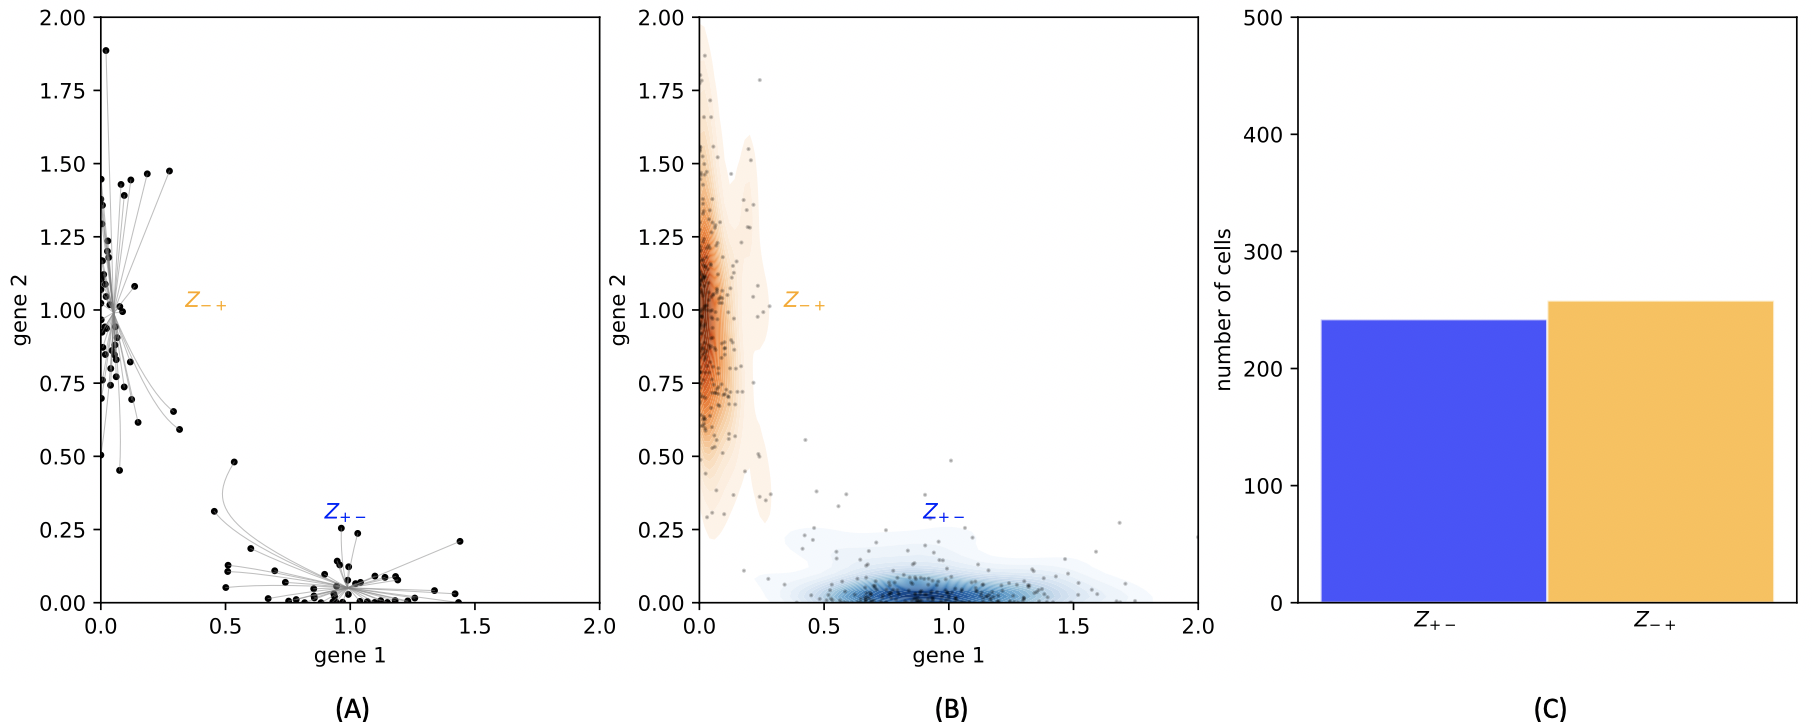
\includegraphics[width=\textwidth]{Images/get_params.png}
    \caption{(A): 100 cells are plotted under the stationary distribution. The relaxation trajectories allow to link every cell to its associated attractor. (B): 500 cells are plotted under the stationary distribution. They are then classified depending on their attractor, and this figure sketches the kernel density estimation of proteins within each basin. (C): The ratio of cells that are found within each basin gives an estimation of the stationary distribution on the basins.}
    \label{fig:discrete_rep}
\end{figure}
\fi

\subsection{Mixture approximation of time-varying distribution}
\label{temporal_mixture}

In the mixture approximation, the marginal on proteins of the stationary distribution of a single cell is characterized by a hidden Markov model: in each basin $z \in Z$, which corresponds to the hidden variable,  the vector $P$ is randomly chosen under the quasistationary distribution $\hat{u}_{z}$ of $X \mid Z = z$. Therefore, the mixture distribution can also be used as a proxy for the time-varying distributions of the bursty model \eqref{model_final}. Denoting $\mu_t$ the distribution on the basins at any time $t$, and considering that a cell reaches almost immediately its quasistationary distribution after entering in a basin, we obtain the approximation:
$$u_t^\theta \approx \sum\limits_{z \in Z}\mu_{t}(z)\prod\limits_{j=1}^n \textrm{Gamma}\left(\frac{k_{z, j}}{d_{1,i}}, c_j\right).$$
In that case, the only time-dependent parameters are the coordinates of the vector $\mu_{t} \in [0,1]^m$ where $m$ is the number of basins, and $\mu_{t}(z) = \mu(z)$ if $t$ is such that the stationary distribution is reached.\\

We remark that with the method described in Figure \ref{fig:discrete_rep}, it would be possible to miss some basins that are important for describing the network, but which would not appear in the stationary distribution. It is expected to be a common situation for networks showing complex behaviours, as feedback loops or unbalanced branching structure, because the probability after a long time may be too weak for some basins to be visited, while playing an important role in the process beforehand. For such networks, the method should then be applied on a serie of timepoints, and the union of all the basins identified at every timepoint should be considered (fixing the value $\mu_t(z) = 0$ for basins $z$ that are not observed at time $t$). In that point of view, the basins appearing in the stationary distribution can be considered as (almost) absorbing states of the coarse-grained model.\\

Altogether the reduction and methods described above establish a formal basis for the definition of a simplified epigenetic landscape given a GRN, under the form of a mixture model. As the mixture parameters seem possible to obtain from a single-cell dataset (see Section \ref{cardamom}), it would be fruitful to use the same formalism to assess the inverse problem of inferring the most likely GRN, given an (experimentally-determined) cell distribution in the gene expression space, a notoriously difficult task \cite{Pratapa_2020}, \cite{herbachinferring2017}. 

